% !TEX root = ../main.tex

\chapter{Results}\label{chapter:results}

Every numeric value reported in this chapter has been recomputed from the saved per-trial prediction arrays or read from the canonical metric files for that trial.\ The chapter follows the natural order: base trial accuracy first, then MC Dropout uncertainty quality, calibration and conformal coverage, post-hoc and proper-scoring diagnostics, ensembles, the three uncertainty-aware extensions, and finally the stratified analysis.

\paragraph{Where the method is weakest -- read this first.}\ Before reporting the headline numbers it is worth flagging the regime in which the proposed UQ pipeline is least reliable, because that regime is also the most policy-relevant.\ Section~\ref{sec:stratified_results} stratifies the test set by $|\Delta v|$ and shows that the ranking quality of MC Dropout weakens substantially on the largest-$|\Delta v|$ quartile (Spearman $\rho$ falls from $0.721$ on Q1 to $0.100$ on Q4, while MAE rises from $1.24$ to $10.08$ veh/h).\ The high Q1 number is partly mechanical, but the Q4 degradation is real: on the segments where the policy intervention has the strongest effect, the uncertainty signal is the least informative.\ For decision support this is the opposite of the regime a planner cares about.\ Because $|\Delta v|$ itself is unobservable at deployment, the recommendations in Section~\ref{sec:deployment} use the two observables that are available -- predicted uncertainty $\sigma$ and the magnitude of the predicted response $|\widehat{\Delta v}|$ -- as proxies, and treat high-uncertainty predictions and predictions with large predicted responses as cases that should be re-simulated in MATSim rather than trusted directly.

\section{Base Trial Performance (T1--T8)}\label{sec:trial_results}

Table~\ref{tab:trial_results} summarises test-set performance.\ T1--T6 are evaluated on 50 test graphs under the 80/15/5 split, while T7 and T8 use 100 graphs under the 80/10/10 split ($3{,}163{,}500$ nodes).\ Because the test sets differ, comparisons across the two groups carry a component that comes from test-set composition rather than from architectural choice, and should be read descriptively.\ Among the trials that combine the GATConv output with non-zero dropout (T2, T5, T6, T7 and T8), T8 is the strongest with $R^2 = 0.5957$, MAE $= 3.957$ veh/h and RMSE $= 7.118$ veh/h.\ T3 and T4 disable dropout entirely and are therefore not MC-Dropout-compatible.\ Trial~1 reaches the highest absolute $R^2 = 0.7860$ but its effective dropout is zero, which makes MC Dropout (the main UQ method studied in the thesis) undefined on it.\ The two weighted-loss runs (T3 and T4) fail to generalise at this data scale, with $R^2$ between $0.22$ and $0.24$.\ The T1-versus-T8 gap is discussed in Section~\ref{sec:t1_vs_t8_limitation}.

\begin{table}[htbp]
\centering
\caption[Test-set performance across the eight base trials]{Test-set performance, recomputed from the saved \texttt{.npz} files.}
\label{tab:trial_results}
\resizebox{\textwidth}{!}{%
\begin{tabular}{lcccccc}
\toprule
Trial & Final layer & Split & Test graphs & $R^2$ & MAE & RMSE \\
\midrule
T1 & Linear & 80/15/5 & 50 & 0.7860 & 2.972 & 5.396 \\
T2 & GATConv & 80/15/5 & 50 & 0.5117 & 4.328 & 8.151 \\
T3 & GATConv & 80/15/5 & 50 & 0.2246 & 5.990 & 10.270 \\
T4 & GATConv & 80/15/5 & 50 & 0.2426 & 6.080 & 10.151 \\
T5 & GATConv & 80/15/5 & 50 & 0.5553 & 4.242 & 7.778 \\
T6 & GATConv & 80/15/5 & 50 & 0.5223 & 4.324 & 8.061 \\
T7 & GATConv & 80/10/10 & 100 & 0.5471 & 4.060 & 7.534 \\
\textbf{T8} & \textbf{GATConv} & \textbf{80/10/10} & \textbf{100} & \textbf{0.5957} & \textbf{3.957} & \textbf{7.118} \\
\bottomrule
\end{tabular}}
\end{table}

\paragraph{T1, T8 and the Deep Ensemble at a glance.}\ Table~\ref{tab:t1_t8_de_compact} sets out the trade-off behind the choice of T8 as the main UQ model.\ T1 has the highest raw test $R^2$ in the project but is not compatible with MC Dropout.\ T8 is the strongest UQ-compatible base, which is the property that matters for the rest of the thesis, but it is not the highest-accuracy model; the Deep Ensemble is.\ Reading the rest of this chapter as a statement about UQ quality on T8, rather than as a statement about the best possible point-prediction surrogate, is therefore the right framing.

\begin{table}[htbp]
\centering
\caption[Compact comparison: T1, T8, Deep Ensemble]{Compact comparison of T1, T8 and the Deep Ensemble.\ T1 has the highest absolute $R^2$ but is not MC-Dropout-compatible; T8 is the primary UQ base; the Deep Ensemble has the highest $R^2$ among the UQ-compatible models.\ T1 was evaluated on a separate 50-graph test set under an 80/15/5 split, whereas T8 and the Deep Ensemble share a different 100-graph test set under the 80/10/10 split (not a subsampled version of the same set), so the two test sets are independent and the cross-group comparison should be read descriptively.}
\label{tab:t1_t8_de_compact}
\resizebox{\textwidth}{!}{%
\begin{tabular}{lcccl}
\toprule
Model & Test graphs & $R^2$ & MC-Dropout-compatible? & Role in this thesis \\
\midrule
T1 & 50 & \textbf{0.7860} & No (effective dropout 0) & Architectural reference; not used for UQ \\
T8 & 100 & 0.5957 & Yes & Primary UQ base model \\
Deep Ensemble & 100 & \textbf{0.6841} & Yes (per member) & Strongest UQ-capable GNN point accuracy \\
\bottomrule
\end{tabular}}
\end{table}

\section{MC Dropout Uncertainty (T8)}\label{sec:mc_results}

MC Dropout with $S = 30$ on the full T8 test set produces pooled Spearman $\rho = 0.4820$ between $\sigma$ and $|y - \hat y|$, with mean $\bar\sigma = 1.369$ veh/h.\ MC-mean accuracy is approximately $0.01$ $R^2$ below the deterministic forward pass ($R^2 = 0.5856$ vs $0.5957$, a difference of $0.0101$), a small expected effect of stochastic averaging.\ The pooled $\rho$ includes the Q1 quartile (zero-effect segments, Section~\ref{sec:stratified_results}); the per-graph mean $0.464$ with bootstrap 95\% CI $[0.460, 0.469]$ is the more conservative summary.\footnote{Cross-trial replication on Trial~7 (dropout 0.3): $\rho = 0.4437$, $k_{95} = 16.15$, AUROC $= 0.7416$ at top-10\% -- qualitatively unchanged.}

\paragraph{Per-graph stability.}\ Per-graph $\rho$ has mean $0.464$, std $0.023$, range $[0.407, 0.505]$.\ A bootstrap ($B = 10{,}000$) gives a 95\% CI of $[0.460, 0.469]$ for the mean per-graph $\rho$.

\paragraph{$S$-convergence.}\label{sec:s_conv_results}\ Convergence on 10 test graphs: $S = 30 \to 50$ adds only $+1.03\%$ in $\rho$ ($0.466 \to 0.471$); $S = 5 \to 30$ contributes $+10.8\%$.\ $S = 30$ is therefore used throughout.

\section{Calibration and Conformal Prediction (T8)}\label{sec:calibration_results}

\noindent\emph{A note on what coverage means in this section.}\ Coverage statements below are \emph{marginal}: PICP is the proportion of test residuals that fall inside the predicted interval averaged across scenarios and nodes on the held-out evaluation split.\ It is not a conditional guarantee for any single scenario or any single uncertainty bin, and node-level predictions inside one graph remain spatially correlated.\ The conditional-coverage range across uncertainty deciles is reported separately later in this section, and the exchangeability assumption that backs the marginal guarantee is examined in Section~\ref{sec:exchangeability}.

The empirical scaling factor $k_p$ (Equation~\eqref{eq:kp}) quantifies the mismatch between raw MC Dropout $\sigma$ and a calibrated Gaussian (Table~\ref{tab:calibration_audit}).\ At the $95\%$ nominal level, $\hat y \pm 1.96\sigma$ covers only $54.85\%$ of residuals: raw MC Dropout is useful as a ranking signal but not as an interval estimator.

\begin{table}[htbp]
\centering
\caption[T8 MC Dropout calibration audit]{T8 empirical $k_p$ vs Gaussian reference, full $3{,}163{,}500$-node test set.}
\label{tab:calibration_audit}
\begin{tabular}{cccc}
\toprule
Nominal $p$ & Empirical $k_p$ & Gaussian $k_p$ & Cov.\ at Gaussian $k_p$ \\
\midrule
50\% & 1.71 & 0.67 & 23.4\% \\
70\% & 3.09 & 1.04 & 33.7\% \\
80\% & 4.55 & 1.28 & 40.1\% \\
90\% & 7.74 & 1.64 & 48.6\% \\
\textbf{95\%} & \textbf{11.66} & \textbf{1.96} & \textbf{54.85\%} \\
\bottomrule
\end{tabular}
\end{table}


Split conformal prediction with 50 calibration and 50 evaluation graphs gives $q_{90} = 9.920$ with empirical $\mathrm{PICP}_{90} = 90.02\%$ and $q_{95} = 14.677$ with $\mathrm{PICP}_{95} = 95.01\%$.\ The empirical marginal coverage on the held-out evaluation graphs is therefore close to the nominal targets.\ The formal conformal coverage guarantee rests on exchangeability, which holds at the scenario level here but is only approximated within a single graph; this is discussed in Section~\ref{sec:exchangeability}.\ Adaptive conformal uses MC Dropout $\sigma$ as a normaliser and yields $q^\text{adapt} = 7.71$ at the $90\%$ level, with empirical global $\mathrm{PICP}_{90} = 89.87\%$, $0.13$ percentage points below the nominal target.

\paragraph{Conditional coverage.}\ Standard conformal can over-cover the low-$\sigma$ nodes and under-cover the high-$\sigma$ nodes; here this shows up as $98.1\%$ coverage on decile D1 and only $59.0\%$ on D10, which is consistent with the impossibility result of Barber~et~al.~\cite{barber2021limits} for distribution-free conditional coverage.\ Adaptive conformal narrows the observed range across deciles to $[83.7\%, 96.4\%]$.

\begin{figure}[htbp]
\centering
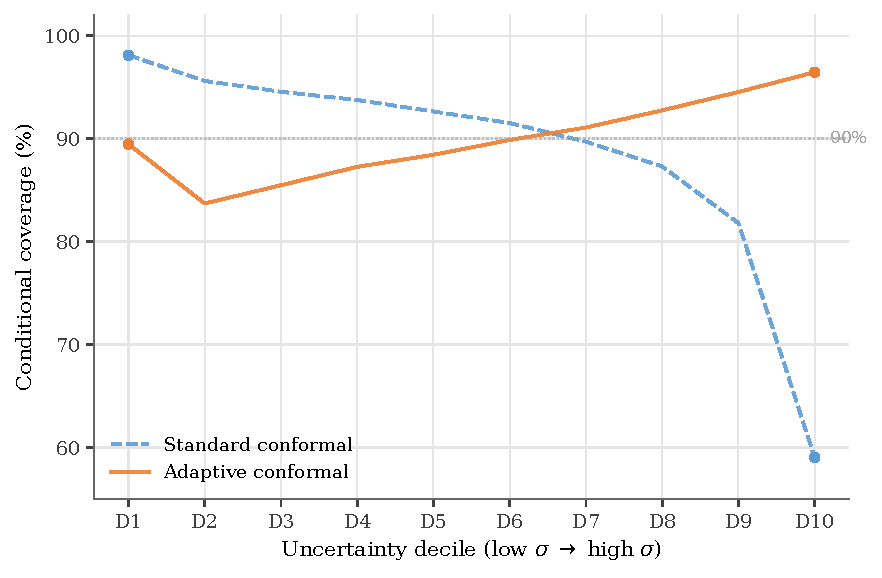
\includegraphics[width=0.85\textwidth]{figures/new/fig15_conditional_coverage_by_decile.pdf}
\caption[Conditional coverage by uncertainty decile]{Standard conformal drifts $39$ pp across deciles; adaptive narrows to $\sim 13$ pp.}
\label{fig:cond_coverage}
\end{figure}

\section{Post-Hoc Regression $\sigma$-Scaling}\label{sec:ts_results}

\paragraph{Motivation.}\ The calibration audit identifies the bulk of the underdispersion as a scale shift in $\sigma$, the failure mode a single-scalar rescaling is designed to correct~\cite{kuleshov2018accurate,laves2020wellcal,levi2022evaluating}; Foong~et~al.~\cite{foong2019between} prove the MC Dropout posterior is too concentrated relative to the exact Bayesian posterior.\ The residual ratios $|y - \hat\mu|/\sigma$ are heavy-tailed (median $1.71$, $p_{99} = 23.6$, max $> 900$), so the Gaussian-NLL closed form $T^{\star 2}_\text{NLL} = N^{-1}\sum (y - \hat\mu)^2/\sigma^2$ returns $T \approx 6.35$ and over-compensates ($1\sigma$ coverage at $86.8\%$).\ The ECE objective targets bulk coverage and is tail-robust; $T^\star_\text{ECE} = 2.887$ hits the $68.3\%$ Gaussian target within $0.3$ pp, and the residual tail mismatch is handled by conformal prediction (Section~\ref{sec:scoring_results}).

Fitting a scalar $T$ on a $30\%$ random node-level calibration subset (seed $42$, $949{,}050$ nodes) gives $T^\star = 2.887$.\ Because this split is at the node level, the calibration and evaluation halves are not strictly independent at the scenario level: nodes within the same graph remain correlated.\ The diagnostics in Table~\ref{tab:temp_scaling} should therefore be read as empirical post-fit coverage rather than as a guarantee at the graph level.\ ECE drops from $0.356$ to $0.034$, a $90.5\%$ reduction; the $1\sigma$ coverage rises from $32.7\%$ to $68.0\%$, which is within $0.3$ pp of the $68.3\%$ Gaussian target; and $k_{95}$ falls from $11.66$ to $4.04$.\ Both before- and after-scaling values of $k_{95}$ are computed on the same held-out $70\%$ evaluation subset, so the comparison is consistent.\ The remaining gaps at $2\sigma$ and $3\sigma$ reflect heavier-than-Gaussian tails: a single scalar can rescale the predictive distribution but cannot reshape it.

\begin{table}[htbp]
\centering
\caption[T8 regression $\sigma$-scaling diagnostics]{Regression $\sigma$-scaling.\ Gaussian targets: $68.27\%$, $95.45\%$, $99.73\%$.}
\label{tab:temp_scaling}
\begin{tabular}{lccc}
\toprule
Metric & Before ($T = 1$) & After ($T = 2.887$) & $\Delta$ \\
\midrule
ECE & 0.356 & \textbf{0.034} & $-90.5\%$ \\
Coverage at $1\sigma$ & 32.7\% & \textbf{68.0\%} & $+35.3$ pp \\
Coverage at $2\sigma$ & 55.6\% & 85.0\% & $+29.4$ pp \\
Coverage at $3\sigma$ & 69.1\% & 91.6\% & $+22.5$ pp \\
$k_{95}$ & 11.66 & \textbf{4.04} & $-7.62$ \\
\bottomrule
\end{tabular}
\end{table}

\begin{figure}[htbp]
\centering
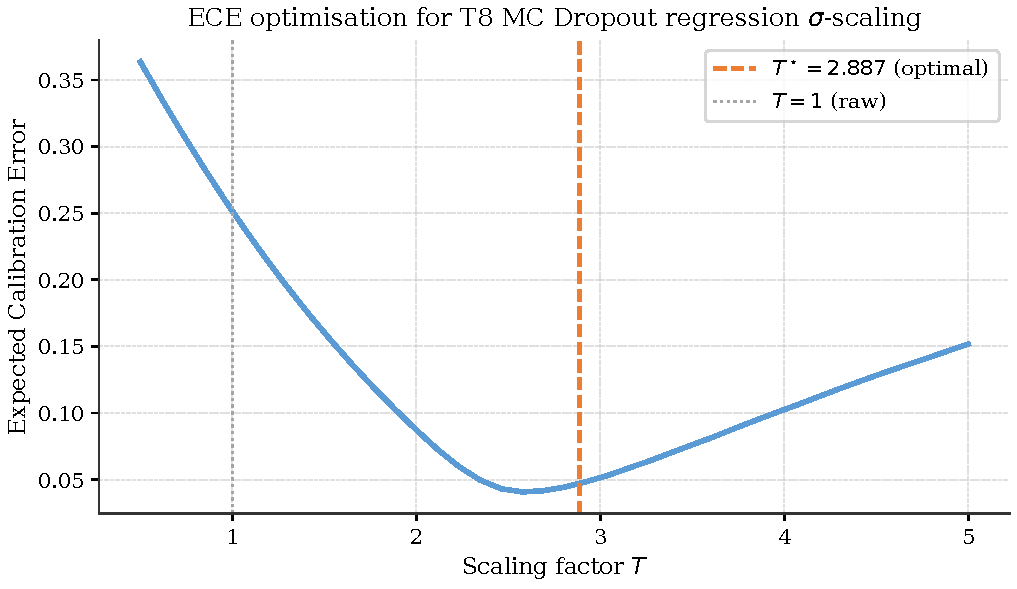
\includegraphics[width=0.75\textwidth]{figures/new/fig12_sigma_scaling_ece.pdf}
\caption[Regression $\sigma$-scaling ECE optimisation]{ECE as a function of the scaling factor $T$ on the calibration subset; the optimum at $T^\star = 2.887$ is marked.\ Coverage and reliability numbers are in Table~\ref{tab:temp_scaling}.}
\label{fig:temp_scaling}
\end{figure}

\section{Proper Scoring Rules, Selective Prediction, Error Detection}\label{sec:scoring_results}

The proper-scoring-rule diagnostics on the full T8 test set are: mean CRPS $= 3.384$ veh/h with CRPS/MAE $= 0.857$ -- the MAE in the denominator is the MC-mean MAE ($3.948$ veh/h, Section~\ref{sec:mc_results}), since CRPS is computed against the MC predictive distribution -- versus the Gaussian-calibrated optimum $1/\sqrt{2} \approx 0.707$; PIT mean $= 0.433$ (ideal $0.500$) and KS $= 0.245$ (ideal $0$); Winkler interval scores at the $90\%$ level $49.68$ for raw MC, $35.78$ for standard conformal ($-28.0\%$), and $\mathbf{32.32}$ for adaptive conformal ($-35.0\%$ vs raw).\ The PIT KS drops to $0.104$ after regression $\sigma$-scaling, but the residual deviation reflects an upward bias in $\hat\mu$ that a scalar rescaling cannot fix: regression $\sigma$-scaling expands the predictive variance symmetrically around $\hat\mu$ and does not shift the predictive centre.\ Conformal prediction is the natural complementary tool here because its intervals expand around $\hat\mu$ to contain the observed residuals, regardless of where $\hat\mu$ itself sits.

\paragraph{Selective prediction.}\label{sec:selective_results}\ Filtering by MC Dropout $\sigma$ percentile and retaining only the most confident fraction yields the curve in Figure~\ref{fig:selective}.\ The 50\% retention point reduces MAE by $41.2\%$ to $2.32$ veh/h; at $25\%$ retention the reduction is $54.5\%$, and at $10\%$ it is $73.4\%$.

\begin{figure}[htbp]
\centering
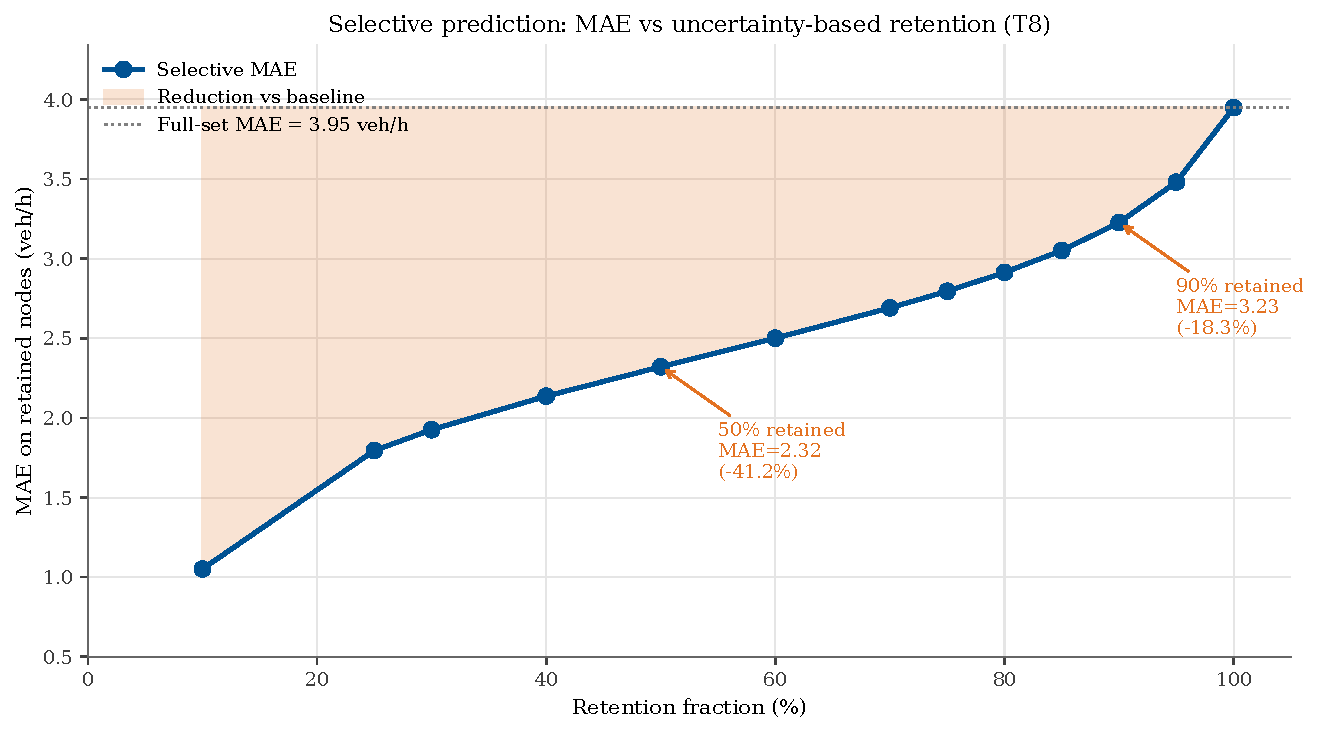
\includegraphics[width=0.9\textwidth]{figures/new/fig07_selective_prediction_curve.pdf}
\caption{Selective prediction curve.\ Annotations mark $50\%$ and $90\%$ retention.}
\label{fig:selective}
\end{figure}

\paragraph{Error detection.}\label{sec:auroc_results}\ Treating $\sigma$ as a classifier of large errors gives an AUROC of $0.7548$ at the top-10\% threshold and $0.7324$ at the top-20\%, both computed on the full $3{,}163{,}500$-node test set.\ Both metrics replicate on Trial~7 ($0.7416$ and $0.7151$; see the footnote in Section~\ref{sec:mc_results}).\ One caveat for both AUROC and the selective-prediction MAE reduction is the high zero-mass in the target: $88.7\%$ of test nodes have $\Delta v = 0$, so a model that predicts near zero with low $\sigma$ is trivially correct for the bulk of the test set; the effect is that AUROC and MAE-on-retained-nodes both look stronger than they would on a balanced subset, and the policy-relevant Q4 stratum (Section~\ref{sec:stratified_results}) remains the more demanding regime.

\section{Ensemble Experiments}\label{sec:ensemble_results}

\paragraph{Single-architecture ensembles (Experiments~A, B).}\ MC Dropout averaged over 5 inference seeds (Experiment~A) gives $\rho = 0.4908$; the seed-ensemble variance gives $\rho = 0.4370$ ($\approx 11.0\%$ relative drop from MC averaging); their quadrature combination gives $\rho = 0.4909$, indistinguishable from MC Dropout alone.\ The multi-model ensemble of T2/T5/T6/T7/T8 (Experiment~B, $R^2$-weighted) gives $\rho = 0.4333$ and $R^2 = 0.5656$, below the best single model (T8, $R^2 = 0.5957$) because averaging across models of uneven quality dilutes the strongest predictor.

\paragraph{Deep Ensemble (Trial D).}\label{sec:deep_ens_results}\ Five PointNetTransfGAT models with T8 hyperparameters and seeds $\{42, 137, 256, 389, 512\}$ form the strongest GNN-based UQ-capable point predictor: $R^2 = \mathbf{0.6841}$ ($+14.8\%$ over T8), MAE $= 3.485$, RMSE $= 6.293$ veh/h.\ Member $R^2$ values lie in $[0.640, 0.650]$, so the ensemble mean exceeds every member.\ Uncertainty signal is weaker than MC Dropout: $\rho = 0.3997$ ($-17.1\%$), $k_{95} = 15.18$.\ Chapter~\ref{chapter:discussion} discusses this complementarity.

\begin{figure}[htbp]
\centering
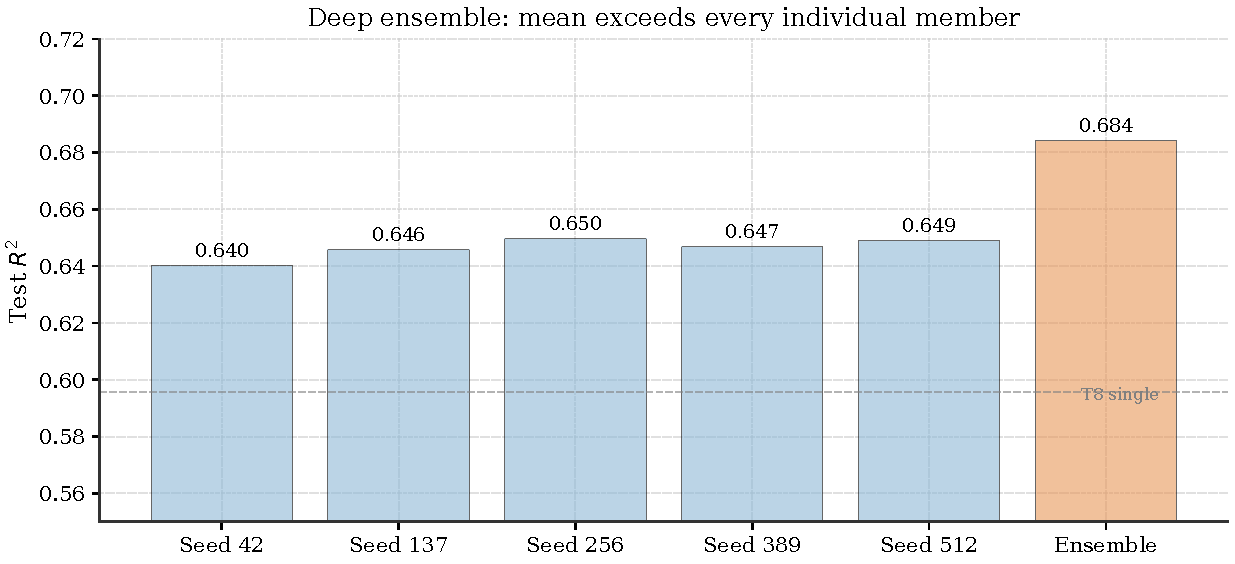
\includegraphics[width=0.85\textwidth]{figures/new/fig26_deep_ensemble_member_r2.pdf}
\caption{Deep Ensemble: mean exceeds every individual member.}
\label{fig:de_member_r2}
\end{figure}

\begin{figure}[htbp]
\centering
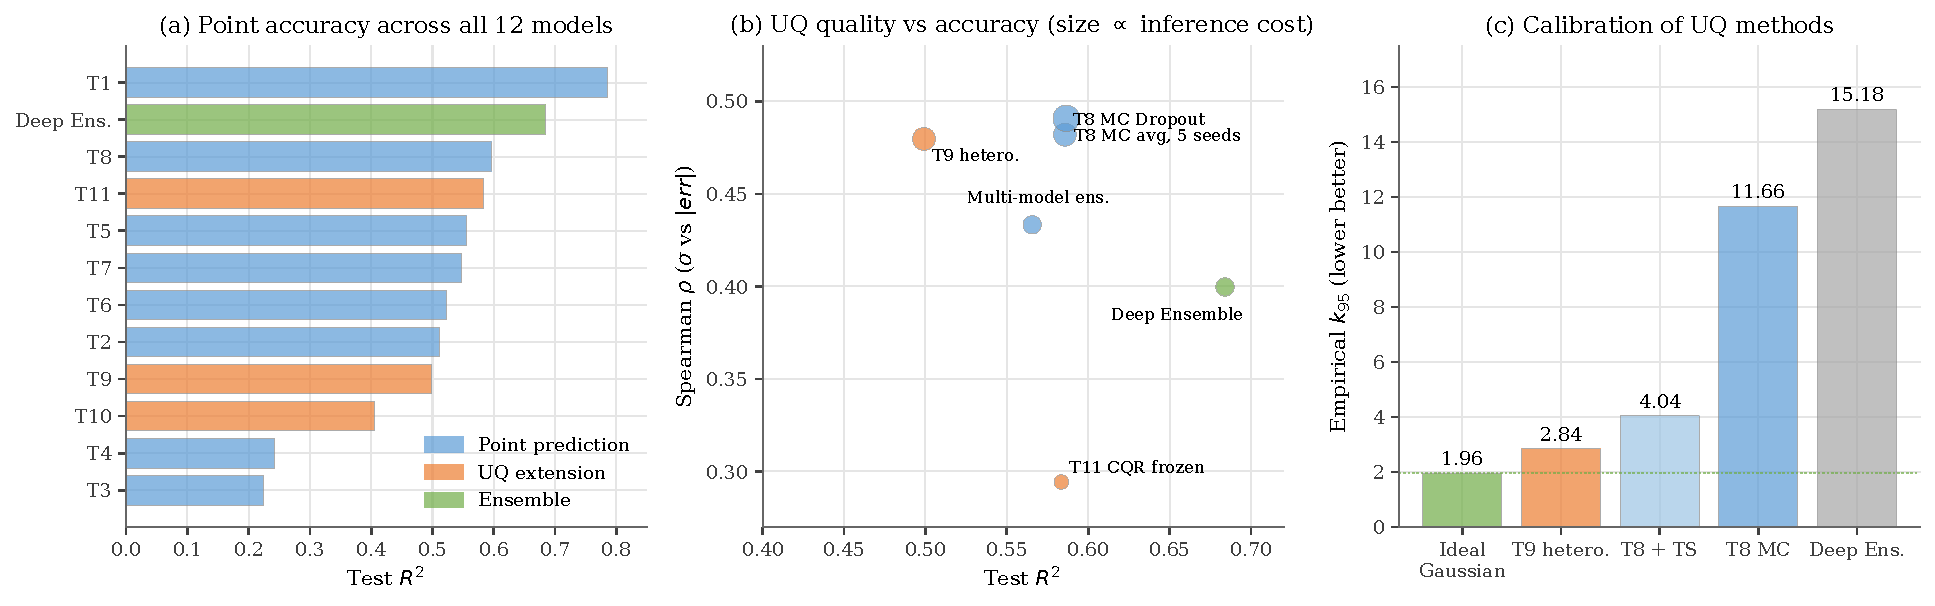
\includegraphics[width=\textwidth]{figures/new/fig00_all_models_summary.pdf}
\caption[Master summary of the GNN-based evaluated models]{Master summary of the twelve GNN-based and uncertainty-aware models evaluated in this thesis.\ Panel (a) sorts trials by test $R^2$ (point-prediction trials blue, uncertainty-aware extensions orange, Deep Ensemble green); the Deep Ensemble leads UQ-compatible models at $R^2 = 0.6841$.\ Panel (b) is the accuracy/UQ trade-off ($R^2$ vs Spearman $\rho$, marker size proportional to $\log$ inference cost): Deep Ensemble and MC Dropout sit on opposite corners; T11 (frozen-backbone CQR) occupies an attractive low-cost corner.\ Panel (c) compares $k_{95}$ (lower is better, Gaussian ideal $1.96$); T9 is closest to ideal among trained models.}
\label{fig:master_summary}
\end{figure}

\section{Trial 9: Heteroscedastic, Frozen Backbone}\label{sec:t9_results}

T9 freezes the T8 backbone and trains only the $134$-parameter heteroscedastic head under Gaussian NLL.\ Two of three gates pass: $\mathrm{PICP}_{90} = 86.90\%$, $\mathrm{PICP}_{95} = 90.01\%$, but $R^2 = 0.4991$ misses the $\geq 0.55$ gate (deterministic single pass: $R^2 = 0.5118$).\ $k_{95}$ improves $4\times$ to $2.84$.\ The $R^2$ miss is consistent with the NLL--MSE trade-off (Section~\ref{sec:hetero_bg}): with a small head, the gradient is reduced more cheaply by inflating $\hat\sigma$ than by improving $\hat\mu$~\cite{seitzer2022pitfalls}.\ The decomposition attributes $99.85\%$ of nodes to the aleatoric component ($\bar\sigma_\text{alea}/\bar\sigma_\text{epi} = 4.24$); whether this reflects genuine traffic-flow variability or NLL-driven $\hat\sigma$ inflation cannot be separated without ground-truth uncertainty labels.

\begin{table}[htbp]
\centering
\caption[Trial 9 gate check]{Trial 9 versus T8 and go/no-go gates.\ The $k_{95}$ row is reported for diagnostic comparison with T8; it is not one of the three Trial~9 gates ($R^2$, PICP$_{90}$, PICP$_{95}$).}
\label{tab:t9_gates}
\begin{tabular}{lcccc}
\toprule
Metric & T8 & T9 & Gate & Status \\
\midrule
$R^2$ (MC mean) & 0.5957 & \textbf{0.4991} & $\geq 0.55$ & \textbf{FAIL} \\
PICP$_{90}$ & 90.02\% & 86.90\% & $\geq 85\%$ & PASS \\
PICP$_{95}$ & 95.01\% & 90.01\% & $\geq 90\%$ & PASS \\
$k_{95}$ (diagnostic) & 11.66 & \textbf{2.84} & lower better & $4\times$ improvement \\
\bottomrule
\end{tabular}
\end{table}

\begin{table}[htbp]
\centering
\caption[Trial 9 aleatoric vs epistemic decomposition]{Trial 9 attributes nearly all predicted uncertainty to the aleatoric component.\ Whether this reflects genuine traffic-flow variability or NLL-driven $\hat\sigma$ inflation~\cite{seitzer2022pitfalls} cannot be separated without ground-truth uncertainty labels.}
\label{tab:t9_decomp}
\begin{tabular}{lc}
\toprule
Quantity & Value \\
\midrule
Mean aleatoric $\bar\sigma_\text{alea}$ (veh/h) & $4.66$ \\
Mean epistemic $\bar\sigma_\text{epi}$ (veh/h) & $1.10$ \\
Ratio $\bar\sigma_\text{alea} / \bar\sigma_\text{epi}$ & $4.24$ \\
Fraction of nodes that are aleatoric-dominated & $99.85\%$ \\
\bottomrule
\end{tabular}
\end{table}

\section{Trial 10: CQR with Unfrozen Backbone (Negative)}\label{sec:t10_results}

Trial~10 fine-tunes the full backbone under the pinball loss at $\tau \in \{0.05, 0.95\}$, inheriting T8's learning rate ($5 \times 10^{-4}$) and the same head, loss, calibration protocol and 80/10/10 split as Trial~11.\ The midpoint $R^2 = 0.4057$ is reported in Table~\ref{tab:t10_gates}; three of the six gates fail.\ The pattern is consistent with pinball gradients reshaping representations that were originally learned for the conditional mean under MSE.

\begin{table}[htbp]
\centering
\caption[Trial 10 gate check]{T10 against the six CQR gates.}
\label{tab:t10_gates}
\begin{tabular}{lcccc}
\toprule
Metric & T8 & T10 & Gate & Status \\
\midrule
$R^2$ (midpoint) & 0.5957 & \textbf{0.4057} & $\geq 0.57$ & \textbf{FAIL} \\
PICP$_{90}$ & 90.02\% & 89.47\% & $\geq 88\%$ & PASS \\
PICP$_{95}$ & 95.01\% & \textbf{91.78\%} & $\geq 93\%$ & \textbf{FAIL} \\
Width$_{90}$ < Width$_{95}$ & --- & $17.78 < 20.02$ & yes & PASS \\
$\hat Q_{90}$ & --- & \textbf{$-0.0011$} & $> 0$ & \textbf{FAIL} \\
$\hat Q_{95}$ & --- & 1.121 & $> 0$ & PASS \\
\bottomrule
\end{tabular}
\end{table}

\section{Trial 11: CQR with Frozen Backbone (Positive)}\label{sec:t11_results}

T11 freezes the T8 backbone and trains only the $134$-parameter quantile head with the same pinball loss, calibration protocol and learning rate as T10.\ All six gates pass (Table~\ref{tab:t11_gates}): $R^2 = 0.5835$ ($\approx 2\%$ below T8), both PICP targets hit to within $0.2$ pp, both conformal corrections positive, widths monotone.\ MAE rises slightly to $4.302$ vs T8's $3.957$ -- the cost of asymmetric calibrated intervals at one deterministic forward pass.\ Since T10 and T11 share head, loss, data, calibration and learning rate, the contrast isolates a single knob (backbone trainability) and gives the strongest evidence in the chapter for the freezing-backbone observation developed in Chapter~\ref{chapter:discussion}.

\begin{table}[htbp]
\centering
\caption[Trial 11 gate check]{T11 passes all six CQR gates.}
\label{tab:t11_gates}
\begin{tabular}{lcccc}
\toprule
Metric & T8 & T11 & Gate & Status \\
\midrule
$R^2$ (midpoint) & 0.5957 & \textbf{0.5835} & $\geq 0.57$ & \textbf{PASS} \\
PICP$_{90}$ & 90.02\% & \textbf{89.82\%} & $\geq 88\%$ & \textbf{PASS} \\
PICP$_{95}$ & 95.01\% & \textbf{94.91\%} & $\geq 93\%$ & \textbf{PASS} \\
Width$_{90}$ < Width$_{95}$ & --- & $17.83 < 24.82$ & yes & \textbf{PASS} \\
$\hat Q_{90}$ & --- & \textbf{0.124} & $> 0$ & \textbf{PASS} \\
$\hat Q_{95}$ & --- & \textbf{3.623} & $> 0$ & \textbf{PASS} \\
\bottomrule
\end{tabular}
\end{table}

\begin{figure}[htbp]
\centering
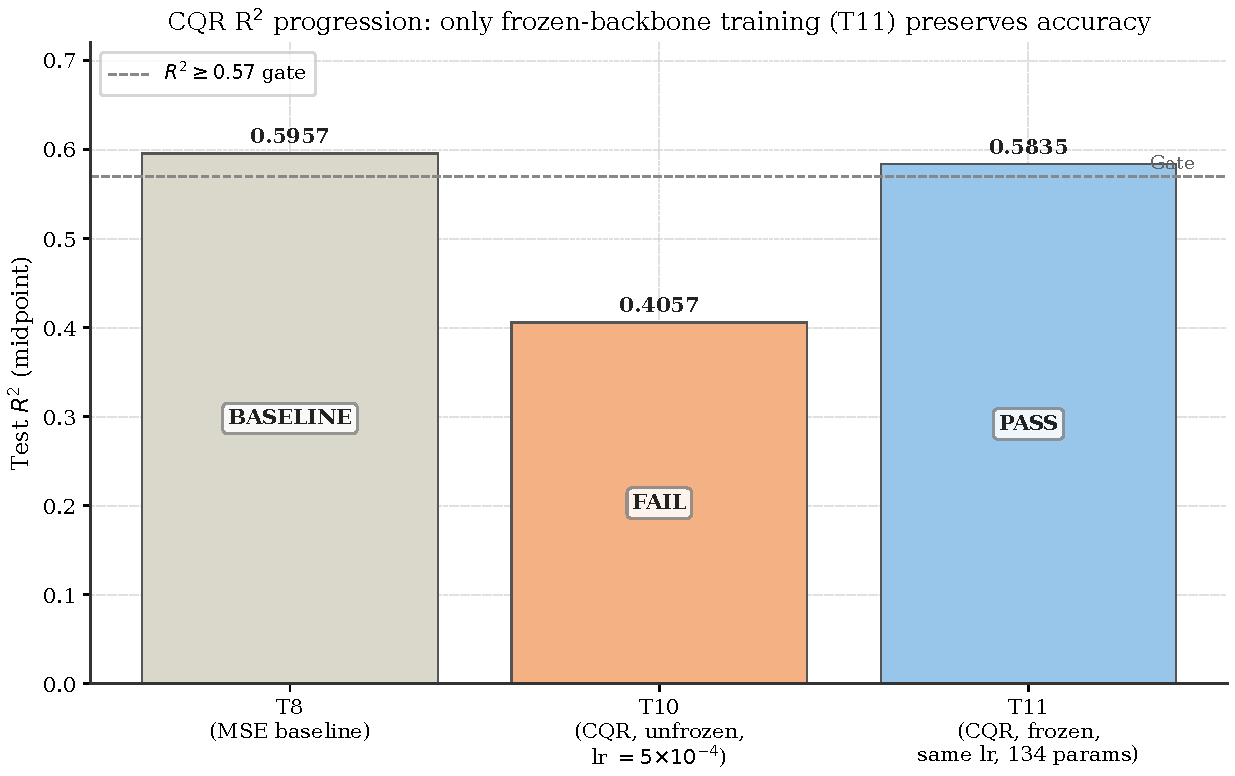
\includegraphics[width=0.9\textwidth]{figures/new/fig22_cqr_r2_progression.pdf}
\caption[CQR $R^2$ progression]{Coefficient of determination across the CQR trials.\ Trial~8 (the MSE-trained baseline) achieves $R^2 = 0.596$.\ Trial~10 with the full backbone unfrozen drops to $R^2 = 0.4057$ and fails the $R^2 \geq 0.57$ gate; Trial~11 with the backbone frozen recovers to $R^2 = 0.5835$ and meets the gate.\ Because T10 and T11 share head, loss, data, calibration protocol and learning rate, the figure highlights backbone trainability as the single design difference between the two and supports the freezing-backbone observation in this experimental setting.}
\label{fig:cqr_r2}
\end{figure}

\section{Stratified UQ by $|\Delta v|$ Quartile}\label{sec:stratified_results}

Rank-based quartiles of $|\Delta v|$ ($790{,}875$ nodes each) show a sharp regime dependence.\ Q1 contains the segments where the policy has no effect at all ($|\Delta v| = 0$ throughout), and Q4 contains the segments with the largest absolute response, up to about $230$ veh/h.\ Within-quartile Spearman $\rho$ between $\sigma$ and $|\text{error}|$ falls from $0.721$ on Q1 to $0.100$ on Q4 (Figure~\ref{fig:stratified}), and MAE rises from $1.24$ to $10.08$ veh/h.\ The high Q1 $\rho$ is partly a mechanical artefact: when $|\Delta v|$ is exactly zero, both $|\text{error}|$ and $\sigma$ reduce to functions of the model's small output magnitude on unchanged segments, and their correlation reflects that shared dependence as much as a genuine ranking signal.\ The substantive degradation on Q4 is real, and the contributing mechanisms are discussed in Section~\ref{sec:stratified_why}.

\begin{figure}[htbp]
\centering
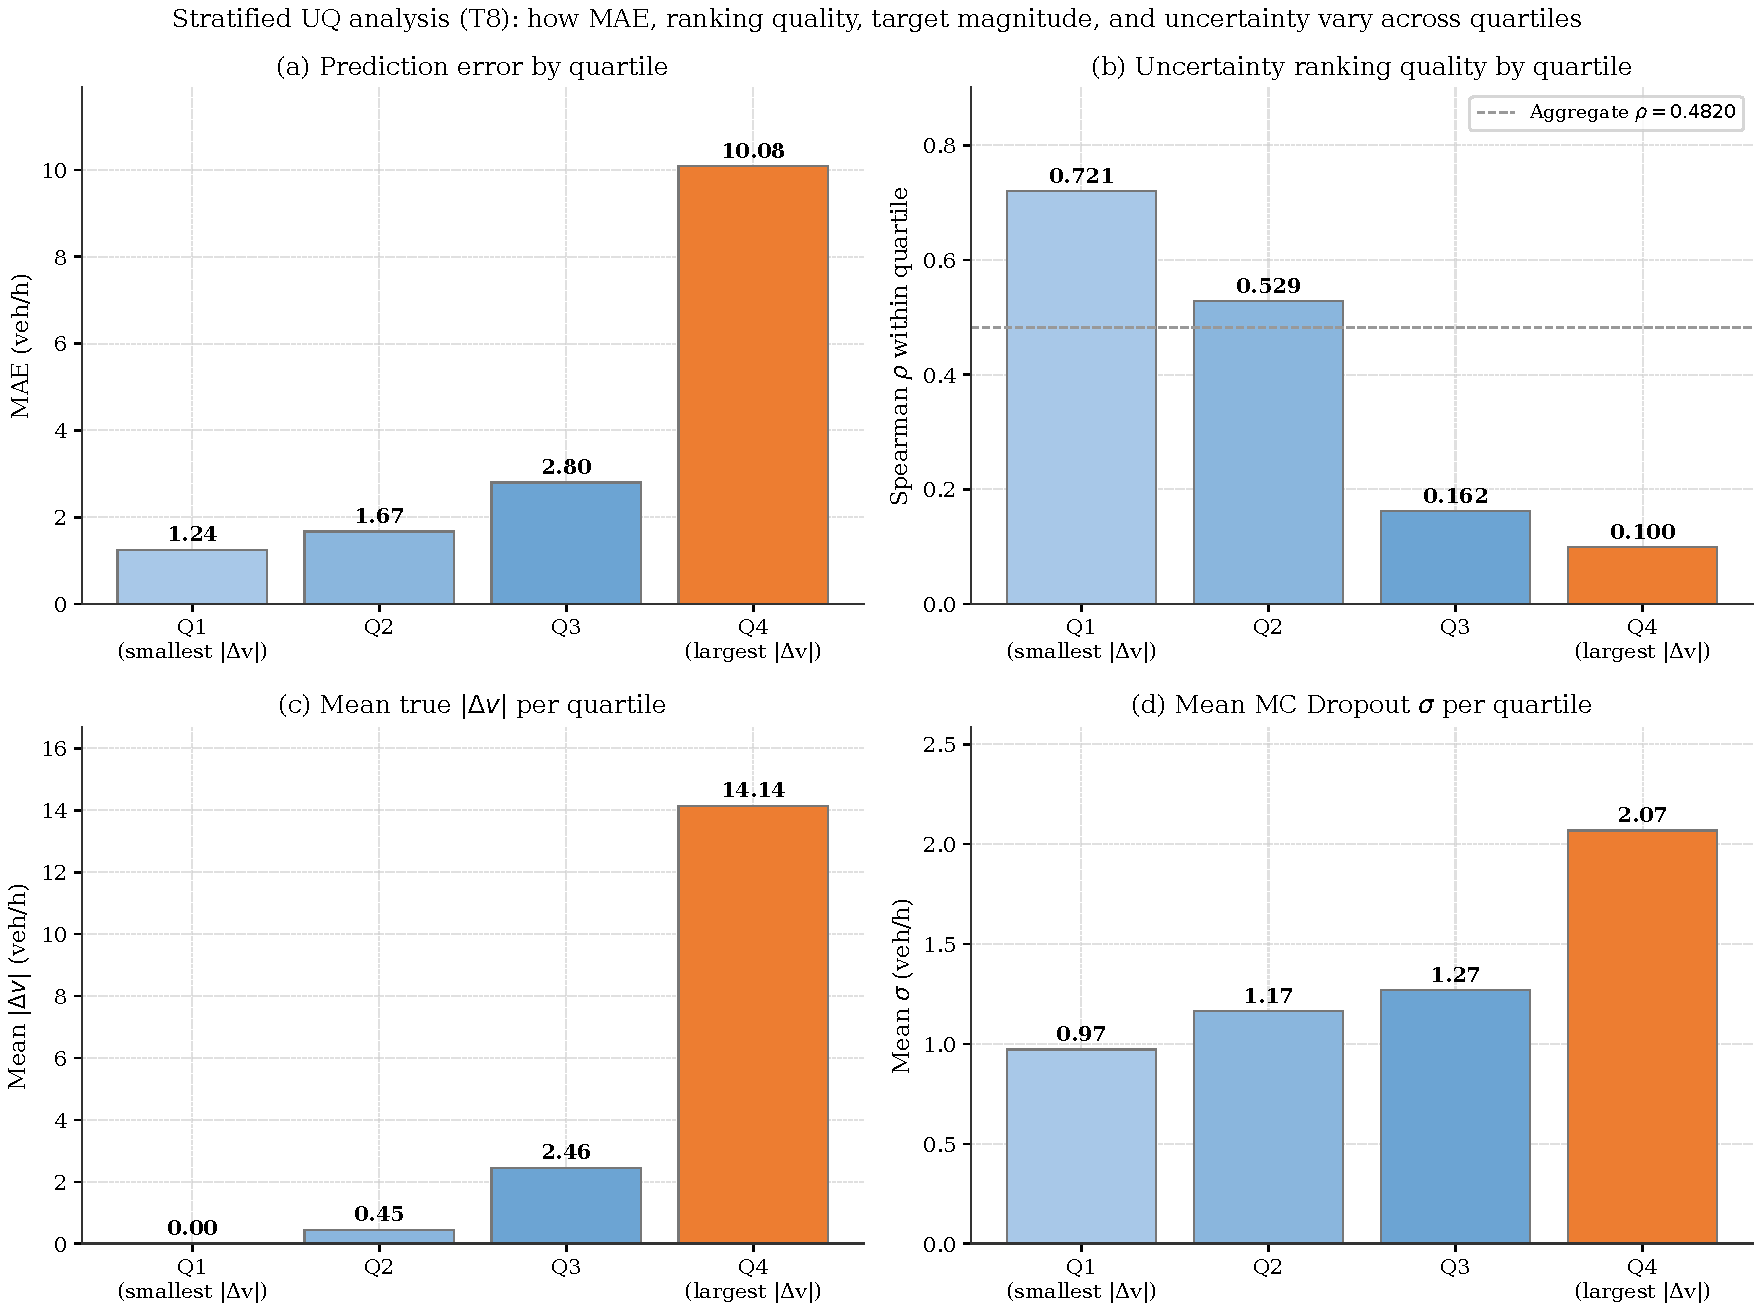
\includegraphics[width=\textwidth]{figures/new/fig28_stratified_uq_quartiles.pdf}
\caption{Stratified UQ: MAE rises and $\rho$ falls as $|\Delta v|$ grows.}
\label{fig:stratified}
\end{figure}

\section{Non-GNN Baselines}\label{sec:non_gnn_baselines}

Three non-GNN baselines on the same five node features and the same scenario-level held-out test set as T8: Random Forest (cuML defaults, $n_\text{est} = 100$, max depth $16$~\cite{breiman2001randomforests}), XGBoost (GPU, default hyperparameters + early-stopping budget of $10{,}000$ rounds on the T8 validation set~\cite{chen2016xgboost}), and a single-hidden-layer MLP (sklearn \texttt{MLPRegressor} architecture~\cite{pedregosa2011scikit}, implemented in PyTorch with AdamW and batch size 4096 for the 25M-row training set).\ All three treat each segment as an independent tabular row, so they do not use the graph topology.\ Both tree baselines exceed T8 on point accuracy (Table~\ref{tab:non_gnn}); the MLP, flat-tabular and without the GNN message passing, falls below T8.

\begin{table}[htbp]
\centering
\caption[Non-GNN baselines vs T8]{Non-GNN baselines on the same 100-graph scenario-level held-out test set ($3{,}163{,}500$ nodes).\ The baselines use default-style configurations from each model's official documentation; XGBoost adds an early-stopping budget on the same scenario-level held-out validation set used by T8, and the MLP is a PyTorch implementation of the sklearn-default architecture with the documented optimisation and batch-size deviations of Section~\ref{sec:non_gnn_baselines}.\ XGBoost \texttt{best\_iteration} reached the $10{,}000$-round budget cap; the validation curve was effectively flat over the last $1{,}000$ rounds and the result is reported at the budget cap rather than at a triggered early stop.}
\label{tab:non_gnn}
\begin{tabular}{lccc}
\toprule
Model & $R^2$ & MAE (veh/h) & RMSE (veh/h) \\
\midrule
T8 (GNN, primary UQ base) & 0.5957 & 3.957 & 7.118 \\
Deep Ensemble (GNN, 5 members) & 0.6841 & 3.485 & 6.293 \\
\midrule
Random Forest (cuML, default-style) & 0.6612 & 3.263 & 6.516 \\
\textbf{XGBoost (default-style + early stop)} & \textbf{0.7414} & \textbf{2.774} & \textbf{5.693} \\
MLP (sklearn-style architecture, PyTorch) & 0.4928 & 3.883 & 7.973 \\
\bottomrule
\end{tabular}
\end{table}

\paragraph{Conformal on Random Forest.}\ Split conformal on the RF point predictions (random 50/50 node-level partition, seed $42$ -- a marginal-coverage sanity check rather than a scenario-level held-out comparison) reaches near-nominal marginal coverage with tighter radii than T8 (Table~\ref{tab:non_gnn_conformal}), reflecting RF's smaller residuals rather than a stronger UQ method.

\begin{table}[htbp]
\centering
\caption[RF + split conformal vs T8 + split conformal]{Split conformal on top of the Random Forest, compared with T8 split conformal from Section~\ref{sec:calibration_results}.\ The RF split is at the \emph{node} level (random 50/50 partition of the 3.16M-node test set, seed $42$), unlike the T8 scenario-level split, so the RF conformal numbers are a marginal-coverage sanity check rather than a scenario-level held-out comparison; see the caveat above.\ Both methods achieve near-nominal marginal coverage on their respective evaluation halves; RF's tighter intervals reflect its smaller residuals, not a stronger uncertainty method.}
\label{tab:non_gnn_conformal}
\begin{tabular}{lcccc}
\toprule
Model & $q_{90}$ (veh/h) & $\mathrm{PICP}_{90}$ & $q_{95}$ (veh/h) & $\mathrm{PICP}_{95}$ \\
\midrule
T8 (GNN) + split conformal & 9.920 & 90.02\% & 14.677 & 95.01\% \\
Random Forest + split conformal & \textbf{8.737} & 89.98\% & \textbf{12.964} & 94.98\% \\
\bottomrule
\end{tabular}
\end{table}

\paragraph{Scope.}\ Tree baselines dominate point accuracy on this sparse target, as expected for tabular data with $88.7\%$ zero-mass response~\cite{grinsztajn2022tree,borisov2022deep}.\ The per-prediction UQ pipeline evaluated in this thesis -- MC Dropout, regression $\sigma$-scaling, the heteroscedastic and CQR heads of Trials~9--11 -- is not directly applicable to the default tree baselines because those methods rely on architectural dropout, soft probabilistic outputs, and a differentiable backbone.\ Tree-native UQ extensions (quantile regression forests, NGBoost) are plausible competitors and a natural follow-up; this thesis does not test them and therefore makes no claim about their relative quality.

\section{An Illustrative Decision Framework}\label{sec:deployment}

Figure~\ref{fig:policy_framework} sketches one way to combine the chapter's findings into an accept/review/reject decision rule based on the predicted $\sigma$ percentile.\ The framework is illustrative: thresholds, costs and risk tolerances would need to be calibrated against the planner's tolerances and the specific decision cost trade-offs before any real deployment.\ The stratified caveat from Section~\ref{sec:stratified_results} also applies: uncertainty ranking weakens on the largest-$|\Delta v|$ segments, exactly the regime where policy effects are biggest; high-impact decisions should still go through MATSim regardless of $\sigma$.

\begin{figure}[htbp]
\centering
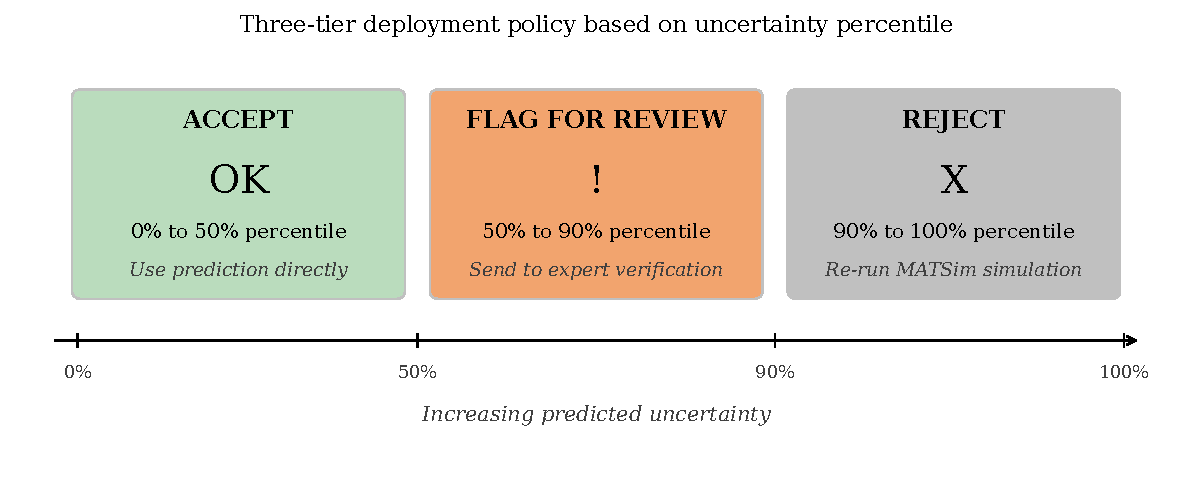
\includegraphics[width=0.7\textwidth]{figures/new/fig35_policy_decision_framework.pdf}
\caption[Illustrative three-tier decision framework]{Illustrative three-tier framework: bottom 50\% accepted ($-41.2\%$ MAE, Fig.~\ref{fig:selective}), middle 40\% reviewed, top 10\% rejected (AUROC $= 0.7548$, Section~\ref{sec:auroc_results}).\ Thresholds need calibration against the planner's cost trade-offs.}
\label{fig:policy_framework}
\end{figure}
